\scanpage{9}
The previous constructions rely heavily on the existence and choice of a field of representatives. Even this being granted, the question of caracterising $Q$ as an actual \uline{sche\`{m}e} \tikz[baseline=(s.base)]{\node[inner sep=0pt](s){,};\node[anchor=south west,inner sep=1pt](a) at ([xshift=-2em,yshift=7pt]s.north west){\inserted{over $k$}};\draw ([xshift=-3pt,yshift=-2pt]s.south west) to[out=90,in=180] ([xshift=0pt,yshift=-2pt]a.south west)--([xshift=0pt,yshift=-2pt]a.south east) to[out=0,in=-90] ([xshift=3pt,yshift=3pt]a.south east);} i.e. as a functor on the category of $k$-algebras, has not been touched. In fact, the description I can give of this functor is \tikz[baseline=(s.base)]{\node[inner sep=0pt](s){in};\node[anchor=south west,inner sep=1pt](a) at ([xshift=-3em,yshift=7pt]s.north west){\inserted{(tautological, and\deleted{)} is )}};\draw ([xshift=-3pt,yshift=-2pt]s.south west) to[out=90,in=180] ([xshift=0pt,yshift=-2pt]a.south west)--([xshift=0pt,yshift=-2pt]a.south east) to[out=0,in=-90] ([xshift=3pt,yshift=3pt]a.south east);} terms of a particular choice of a resolution $X$, and it really gives \deleted{rather} a description pf $P$ rather than $Q$. \deleted{To} One then still has to define $Q$ as the cokernel of the silly morphism $\underline{D}\handwritten{\longrightarrow}P$. As a matter of fact, even if we restrict to argument\unsure{s} $k'$ which are, say, finite extensions of $k$ (but not necessarily separabl\unsure{e} ones), I cannot describe $Q(k')$ in terms of local Picard groups of local rings as $A'=A\mathord{\tikz[baseline=(s.base)]{\node[inner sep=0pt](s){$\mathrm{x}$};\draw[line width=.5pt] ([xshift=.5pt,yshift=1.3pt]s.center) ellipse[x radius=3pt,y radius=4.5pt];}}_k k'$. The trouble, of course, is that $X\mathord{\tikz[baseline=(s.base)]{\node[inner sep=0pt](s){$\mathrm{x}$};\draw[line width=.5pt] ([xshift=.5pt,yshift=1.3pt]s.center) ellipse[x radius=3pt,y radius=4.5pt];}}_k k'$ will in general no longer be a resolution of $S'$, i.e. it will no longer be regular. However, such geometric descriptions will be possible provided we take as arguments algebras which are \tikz[baseline=(s.base)]{\node[inner sep=0pt](s){\deleted{smooth of formally}};\node[anchor=south west,inner sep=0pt] at ([yshift=2pt]s.north west){\inserted{\handwritten{geometrically regular}}};} \deleted{smooth} over $k$, so \deleted{taht} that tensoring with them will not destroy the regularity of $X$. (Thus, the case when $k'$ is a power series ring, for instance the completion of the local ring of $Q$ at the origin, $Q$ being smooth, is of interest ...) Let's now try to be specific. By definition \tikz[baseline=(s.base)]{\node[inner sep=0pt](s){for};\node[anchor=south west,inner sep=1pt](a) at ([xshift=-2em,yshift=7pt]s.north west){\inserted{\handwritten{more or less,}}};\draw ([xshift=-3pt,yshift=-2pt]s.south west) to[out=90,in=180] ([xshift=0pt,yshift=-2pt]a.south west)--([xshift=0pt,yshift=-2pt]a.south east) to[out=0,in=-90] ([xshift=3pt,yshift=3pt]a.south east);} any \tikz[baseline=(s.base)]{\node[inner sep=0pt](s){scheme};\node[anchor=south west,inner sep=1pt](a) at ([xshift=0em,yshift=7pt]s.north west){\inserted{\handwritten{affine}}};\draw ([xshift=-3pt,yshift=-2pt]s.south west) to[out=90,in=180] ([xshift=0pt,yshift=-2pt]a.south west)--([xshift=0pt,yshift=-2pt]a.south east) to[out=0,in=-90] ([xshift=3pt,yshift=3pt]a.south east);} $T$ over $k$, we have
\margin{\figure{\handwritten{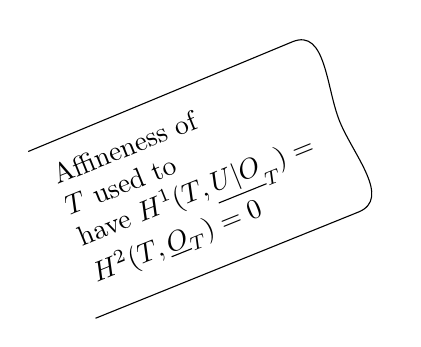
\begin{tikzpicture}[rotate=22,transform shape]
\node[inner sep=2pt,align=left](s){Affineness of\\$T$ used to\\have $H^1(T,\underline{\unsure{U|O}}_T)=$\\$H^2(T,\underline{O}_T)=0$};
\draw[line width=.4pt] ([xshift=-.3em,yshift=.6em]s.north west)--([xshift=.5em,yshift=.7em]s.north east) to[out=0,in=90] ([xshift=1em]s.east) to[out=-90,in=0] ([xshift=.4em,yshift=-.7em]s.south east)--([xshift=-.3em,yshift=-.7em]s.south west);
\end{tikzpicture}}}}
\[
\begin{aligned}
\handwritten{(18)}\qquad\qquad & P(T)=\underset{\handwritten{\longleftarrow}}{\lim}P_n(T)\handwritten{\hookleftarrow}\underset{\handwritten{n}}{\underset{\handwritten{\longleftarrow}}{\lim}}\operatorname{Pic}(X_{n_T}\deleted{\unsure{,\underline{O}_{X_{nT}}}})\handwritten{/\operatorname{Pic}\mathord{\tikz[baseline=(s.base)]{\node[inner sep=0pt](s){$(T)$};\fill ([xshift=-1pt,yshift=-5pt]s.south east) circle (.3pt);}}}\qquad (X_{n\,T}=X_n\mathord{\tikz[baseline=(s.base)]{\node[inner sep=0pt](s){$\mathrm{x}_{\unsure{\mathbb{k}|k}}$};\fill ([xshift=-.4em,yshift=-.25em]s.center) circle (.3pt);\fill ([xshift=-.5em,yshift=-.55em]s.center) circle (.3pt);}} T)\ .
\end{aligned}
\]
In fact, it is not hard to check that the left hand side functor is the étale sheaf (on $(\mathrm{Sch})_{/k}$): associated to the \deleted{left ha\unsure{n}} right-hand side functor. This comes from the more \tikz[baseline=(s.base)]{\node[inner sep=0pt](s){precise};\fill ([xshift=1pt,yshift=-2pt]s.south west) circle (.3pt);\fill ([xshift=3pt,yshift=-2pt]s.south west) circle (.3pt);} statement that the obstruction, for an element of $P(T)$, to come from an element of $\deleted{\operatorname{Pic}(X_{\unsure{nT|2T}})}\underset{\handwritten{n}}{\underset{\handwritten{\longleftarrow}}{\lim}}\operatorname{Pic}(X_{nT})$, lies in $H^2(T_{\text{ét}},\underline{G}_m)$ \handwritten{(} at least for $T$ affine, \deleted{\handwritten{(}}which is used to insure that it's $H^{\unsure{\rlap{$\scriptstyle1$}\handwritten{2}|\rlap{$\scriptstyle2$}\handwritten{1}}}$ and $H^{\unsure{\rlap{$\scriptstyle2$}\handwritten{3}|\rlap{$\scriptstyle3$}\handwritten{2}}}$ with values in $\underline{O}_T$ vanish\deleted{\handwritten{)}}, For simplicity, I have assumed here that $A$ is normal\handwritten{)}. As \tikz[baseline=(s.base)]{\node[inner sep=0pt](s){we};\draw[line width=.45pt] ([xshift=-.5em,yshift=.3em]s.south east) to[out=180,in=90] ([xshift=-.6em,yshift=-.08em]s.south east) to[out=-90,in=180] ([xshift=.4em,yshift=-.15em]s.south east);} have seen
% archive sheet number: 8
